% !TeX program = lualatex
% !TeX root = luaking.tex
% !TeX encoding = UTF-8
% !TeX spellcheck = cs_CZ
%---------------------------------------------------------------------------------------------------
% file fey1ch11.tex
%---------------------------------------------------------------------------------------------------
%================= Kapitola: Vektory ===============================================================
\setchaptertoc
\chapter{Vektory}\label{fyz:IchapXI}
  \section{Symetrie ve fyzice}
    V této kapitole zavedeme pojem, jenž je ve fyzice známý jako \emph{symetrie fyzikálních 
    zákonů}. Slovo \uv{symetrie} tu používáme ve zvláštním smyslu, a proto bude třeba ho definovat. 
    Je-li nějaká věc symetrická - jak to můžeme definovat? Říkáme-li, že obraz je symetrický, 
    rozumíme tím, že jeho jedna strana je nějak stejná jako druhá. Profesor Hermann Weyl definoval 
    symetrii takto: Předmět je symetrický, můžeme-li ho podrobit určité operaci a po ní bude stejný 
    jako původně. Například, podíváme-li se na vázu, jež má pravo-levou symetrii, pak otočením o 
    \qty{180}{\degree} kolem vertikální osy bude vypadat opět stejně. Přijmeme Weylovu obecnější 
    definici symetrie a na jejím základě budeme hovořit o symetrii fyzikálních zákonů.
    
    Předpokládejme, že na určitém místě jsme postavili složité zařízení s množstvím interakcí, se
    srážejícími se kuličkami, mezi nimiž působí síly atd. Dále předpokládejme, že na jiném místě
    jsme vybudovali přesně stejné zařízení, jehož všechny části jsou shodné se stejnými rozměry a
    stejnou orientací - vše je stejné, jen je to posunuto o určitou vzdálenost. Ptáme se, zda se
    budou tato zařízení chovat úplně stejně, jestliže je, uvedeme do činnost za stejných počátečních
    podmínek? Budou všechny pohyby paralelní? Odpověď může být samozřejmě záporná, neboť místo pro
    druhé zařízení může být nevhodně zvoleno. Zvolíme-li toto místo někde u stěny, druhé zařízení
    nebude moci vůbec pracovat, neboť stěna při některých pohybech překáží.
    
    Naše fyzikální úvahy vyžadují určitý zdravý smysl při jejich aplikaci, vždyť to nejsou čistě 
    matematické nebo abstraktní myšlenky. Musíme vědět, co to znamená, když hovoříme, že při 
    přesunu zařízení na nové místo pozorujeme stejné jevy. Znamená to, že přemisťujeme vše, co může 
    mít na pohyb vliv. Nepozorujeme-li stejný jev, pak jsme něco důležitého nepřemístili a budeme 
    muset zjistit, co to je. Nezjistíme-li to nikdy, pak můžeme prohlásit, že fyzikální zákony 
    nemají takovou symetrii. Mají-li však fyzikální zákony takovou symetrii, pak příčinu neshody 
    můžeme najít - a my doufáme, že ji najdeme. Například, jestliže se pozorně rozhlédneme, můžeme 
    zjistit, že stěna působí na naše zařízení. Základní otázkou je, zda při dostatečně dobře 
    definovaných poměrech, při započtení všech podstatných sil a přesunu všech důležitých částí na 
    jiné místo budou zákony stejné. Bude zařízení pracovat stejně?
    
    Je jasné, že chceme přesunout celé zařízení a všechny \emph{podstatné} vlivy, ale ne 
    \emph{všechno} na světě - planety, hvězdy a všechno ostatní. Kdybychom totiž přesunuli všechno, 
    měli bychom stejný jev jako původně z toho prostého důvodu, že bychom se ocitli na stejném 
    místě. \emph{Všechno} tedy nemůžeme přesunout. V praxi se ukazuje, že při rozumném výběru 
    přesouvaných věcí bude zařízení pracovat stejně. Jinými slovy, nenarazíme-li na stěnu, 
    budeme-li znát původ vnějších sil a zabezpečíme i jejich přesun, pak bude zařízení pracovat na 
    obou místech stejně.
    
  \section{Translace}\label{fyz:IchapXIsecI}
    V našich úvahách se omezíme na mechaniku, o níž toho víme již dost. V předcházející kapitole
    jsme poznali, že zákony mechaniky je možné shrnout do tří rovnic pro každou částici
    \begin{equation}\label{fyz:eq145}
      m\dder{x}{t} = F_x, \;
      m\dder{y}{t} = F_y, \;
      m\dder{z}{t} = F_z.
    \end{equation}

    \begin{figure}[ht!]  %\ref{fyz:fig0113}
      \centering
      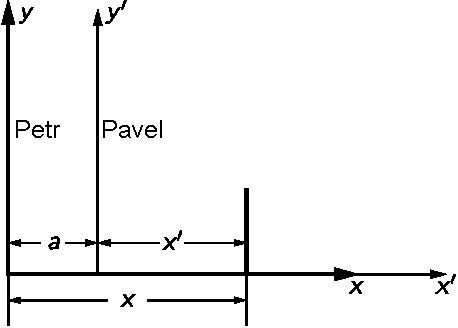
\includegraphics[width=0.8\linewidth]{fyz_fig0113.pdf}
      \caption{Dvě paralelní soustavy souřadnic (\cite[s.~154]{Feynman01})}
      \label{fyz:fig0113}
    \end{figure}
    To znamená, že existuje způsob měření vzdáleností \(x, y, z\) na třech navzájem kolmých osách i
    sil podél těchto směrů, a při takovém měření jsou rovnice (\ref{fyz:eq145}) pravdivé. Měření
    musí být realizována od nějakého počátku a my se ptáme, \emph{kde má být tento počátek}. Newton
    by nám řekl jen tolik, že takové místo, ze kterého je možné začít měřit, existuje - snad je to
    střed vesmíru - a při takovém měření jsou uvedené zákony správné. Snadno však nahlédneme, že
    takový střed nikdy nenajdeme, protože nic by se nezměnilo, kdybychom si zvolili jiný počátek.
    Předpokládejme, že existují dva lidé - Petr, který si zvolil počátek na jednom místě, a Pavel,
    který má paralelní soustavu s počátkem na jiném místě (obr. \ref{fyz:fig0113}). Při měření polohy
    bodu v prostoru zjistí Petr, že má souřadnice \(x\), \(y\) a \(z\) (obvykle budeme vynechávat
    \(z\), abychom se vyhnuli komplikacím při kreslení obrázků). Když měří polohu stejného bodu
    Pavel, zjistí, že má hodnotu \(x\) (pro rozlišení ji budeme označovat \(x'\)) a obecně jinou
    hodnotu \(y\), ačkoli v našem příkladu jsou tyto hodnoty číselně stejné. Máme tedy
    \begin{equation}\label{fyz:eq146}
      x' = x - a, \quad y' = y, \quad z' = z.
    \end{equation}
    Aby byla naše analýza úplná, musíme vědět, jaké síly naměří Pavel. Síla působí podél nějaké 
    přímky a silou ve směru osy \(x\) rozumíme tu část z celkové síly, jež působí podél osy \(x\) a 
    získáme ji tak, že násobíme velikost síly kosinem úhlu, který svírá s osou \(x\). Tak 
    zjišťujeme, že Pavel bude mít stejné průměty jako Petr a máme proto soustavu rovnic
    \begin{equation}\label{fyz:eq147}
      F_{x'} = F_x, \quad F_{y'} = F_y, \quad F_{z'} = F_z.
    \end{equation}
    Tyto rovnice představují vztahy mezi veličinami, které vidí Petr a Pavel.
    
    Položme si otázku: Zná-li Petr Newtonovy zákony a snaží-li se Pavel objevit zákony pohybu, 
    budou tyto jeho zákony shodné s Newtonovými? Projeví se nějak změněná volba počátku? Jinak 
    řečeno, jsou-li rovnice (\ref{fyz:eq145}) správné a rovnice (\ref{fyz:eq146}) a 
    (\ref{fyz:eq147}) představují vztahy mezi měřenými veličinami, platí, nebo neplatí následující 
    vztahy?
    \begin{flalign}\label{fyz:eq148}
      m\dder{x'}{t} = F_{x'}, \;
      m\dder{y'}{t} = F_{y'}, \;
      m\dder{z'}{t} = F_{z'}. &&
    \end{flalign}
    Abychom tyto rovnice prověřili, derivujeme dvakrát vztah pro \(x'\). Nejprve dostaneme
    \begin{equation*}
      \der{x'}{t} =\der{ }{t}(x-a) = \der{x}{t} - \der{a}{t}.
    \end{equation*}
    Budeme předpokládat, že Pavlův počátek je pevný, nepohybuje se vzhledem k Petrovu počátku. 
    Proto je \(a\) konstanta a \(da/dt=0\), takže máme
    \begin{equation*}
      \der{x'}{t} = \der{x}{t} \quad\text{a dále}\quad \dder{x'}{t} = \dder{x}{t}.
    \end{equation*}
    Protože předpokládáme, že hmotnosti měřené Petrem a Pavlem jsou stejné, získá rovnice 
    (\ref{fyz:eq148}) pro osu \(x\) tvar
    \begin{equation*}
      m\dder{x}{t} = F_{x'}.
    \end{equation*}
    Součin hmotnosti a zrychlení je tedy u obou pozorovatelů stejný. Získali jsme i vztah pro 
    \(F_{x'}\), neboť po dosazení do rovnice (\ref{fyz:eq145}) zjistíme, že
    \begin{equation*}
      F_{x'} = F_{x}.
    \end{equation*}
    
    Zákony, jež odvodí Pavel, vypadají tedy stejně jako Petrovy. I pro něho platí Newtonovy zákony, 
    i když s jinými souřadnicemi. To znamená, že neexistuje střed vesmíru a pohybové zákony budou 
    stejné bez ohledu na místo, z něhož pozorujeme.
    
    Platí i následující tvrzení: Je-li na určitém místě zařízení obsahující jistý mechanizmus, pak
    stejné zařízení bude na jiném místě pracovat stejné. Proč? Protože zařízení analyzované Pavlem
    vyhovuje stejným rovnicím jako zařízení analyzované Petrem. Protože jsou rovnice stejné, budou
    stejné i jevy. Důkaz toho, že zařízení se na novém místě chová stejně jako na původním, je
    stejný jako důkaz toho, že rovnice přenesené na jiné místo prostoru se reprodukují. Můžeme tedy
    prohlásit, že \textbf{fyzikální zákony jsou symetrické vzhledem k translaci v prostoru},
    symetrické v tom smyslu, že zákony se nemění při translaci soustavy souřadnic. Že je to pravda,
    je celkem zřejmé intuitivně, ale je zajímavé a zábavné se zabývat matematickou stránkou této
    záležitosti. K problému se ještě vrátíme v kapitole \ref{vol03:fyz:IchapXVsecIII}, ve které se
    budeme zabývat \textbf{principem relativity}. 
    
  \section{Rotace}\label{fyz:IchapXIsecII}
    Předcházející část byla věnována první z řady stále komplikovanějších tvrzení týkajících se 
    symetrie fyzikálních zákonů. Další tvrzení praví, že nezáleží na tom, v jakém \emph{směru} 
    zvolíme souřadnicové osy. Jinými slovy, postavíme-li někde jedno zařízení a v sousedství 
    stejné zařízení, ale pootočíme ho o určitý úhel vzhledem k prvnímu zařízení, ptáme se, zda 
    budou obě dvě zařízení pracovat stejně. Určitě nebudou, jsou-li takovým zařízením, například, 
    dědečkovy kyvadlové hodiny! Je-li kyvadlo ve svislé poloze, hodiny spolehlivě pracují, ale 
    nakloníme-li hodiny, kyvadlo narazí na stěnu pouzdra a hodiny se zastaví. V případě kyvadlových 
    hodin je naše tvrzení nesprávné, pokud do zařízení nezahrneme i Zemi, jež působí na pohyb 
    kyvadla. Věříme-li, že fyzikální zákony jsou symetrické vzhledem k rotaci, musíme připustit, že 
    na chod kyvadlových hodin má vliv i něco jiného než kyvadlový stroj, něco mimo hodiny, a my to 
    musíme najít. Ještě můžeme předpovědět, že kyvadlové hodiny nebudou pracovat stejně, budou-li 
    umístěny na různých místech, vzhledem k tomu záhadnému zdroji asymetrie, jímž je snad Země. 
    Skutečně, kyvadlové hodiny umístěné například na umělé družici Země, nepůjdou, neboť tam není 
    efektivní síla a na Marsu by zase měly jinou rychlost. Kyvadlové hodiny \emph{představují} něco 
    více než jednoduchý mechanizmus v jejich vnitřku, zahrnují i něco, co je mimo ně. Známe-li 
    tento faktor, pochopíme, že bychom museli společně s celým zařízením pootočit i Zemi. Nemusíme 
    si však dělat starosti s pootočením Země, stačí chvíli počkat a Země se pootočí sama; pak 
    půjdou kyvadlové hodiny v nové poloze stejně jako předtím. Zatímco rotujeme v prostoru, mění se 
    absolutně i naše úhly; tyto změny nás však příliš neznepokojují, neboť v nové poloze se cítíme 
    stejně dobře jako ve staré. Taková situace nás může zmýlit. V nové pootočené poloze jsou sice 
    zákony stejné jako před pootočením, \emph{není však pravda}, že by \emph{po dobu otáčení} věci 
    podléhaly stejným zákonům, jako když se neotáčejí. Uskutečníme-li dostatečně přesné 
    experimenty, můžeme zjistit, zda Země \emph{rotuje}, ale nemůžeme zjistit, zda Země 
    \emph{rotovala}. Jinými slovy, takto nemůžeme zjistit její orientaci, ale jen skutečnost, že 
    tato orientace se mění.

    \begin{figure}[ht!]  %\ref{fyz:fig0114}
      \centering
      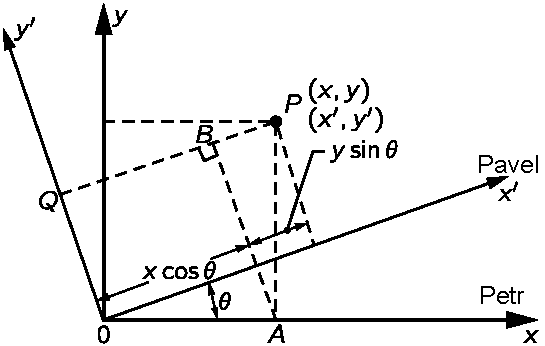
\includegraphics[width=0.8\linewidth]{fyz_fig0114.pdf}
      \caption{Dvě soustavy souřadnic s různou úhlovou orientací
              (\cite[s.~156]{Feynman01})}
      \label{fyz:fig0114}
    \end{figure}
    Nyní uvažujme vliv úhlové orientace na fyzikální zákony. Zjistíme, jak to bude nyní s Petrem a 
    Pavlem. Abychom vyloučili zbytečné komplikace, budeme předpokládat, že Petr i Pavel vycházejí 
    ze společného počátku (již jsme ukázali, že jejich souřadnicové systémy se mohou translací 
    přesunout na jiné místo). Předpokládejme, že Pavlovy osy se pootočily vzhledem k Petrovým osám 
    o úhel \(\vartheta\). Omezíme-li se na dvojrozměrný prostor, můžeme dvě takové soustavy 
    souřadnic znázornit jako na obr. \ref{fyz:fig0114}. Uvažujme nějaký bod \(P\), jež má v Petrově 
    soustavě souřadnice \((x, y)\) a v Pavlově soustavě souřadnice \((x' y')\). Podobně jako v 
    předcházejícím případě, začneme tím, že vyjádříme souřadnice \(x', y'\) pomocí \(x, y\) a 
    \(\vartheta\). Abychom to mohli realizovat, vedeme nejprve kolmice z \(P\) ke všem čtyřem osám 
    a nakreslíme \(AB\) kolmo k \(PQ\). Z obrázku je vidět, že \(x'\) lze vyjádřit jako součet dvou 
    úseček podél osy \(x'\) a \(y'\) zase jako rozdíl dvou úseček podél \(AB\). Délky těchto úseček 
    jsou vyjádřeny pomocí \(x, y\) a rovnicích (\ref{fyz:eq149}), k nimž připojíme rovnici pro 
    třetí rozměr

    \begin{subequations}\label{fyz:eq149}
      \begin{align}
        x' &= x\cos\vartheta + y\cos\vartheta, \label{fyz:eq149a} \\
        y' &= y\cos\vartheta - x\sin\vartheta, \label{fyz:eq149b} \\
        z' &= z.
      \end{align}
    \end{subequations}

    Dalším krokem je analýza vztahů mezi silami naměřenými dvěma pozorovateli, kterou provedeme 
    podobně jako v předchozím případě. Předpokládejme, že síla \(F\), kterou jsme již analyzovali, 
    má složky \(F_x\) a \(F_y\) (při Petrově pozorování) a působí na částici o hmotnosti \(m\), 
    nacházející se v bodě \(P\) (obr. \ref{fyz:fig0114}). Pro zjednodušení posuňme obě souřadnicové 
    soustavy tak, že počátek bude v bodě \(P\) (obr. \ref{fyz:fig0115}).
    
    \begin{figure}[ht!]  %\ref{fyz:fig0115}
      \centering
      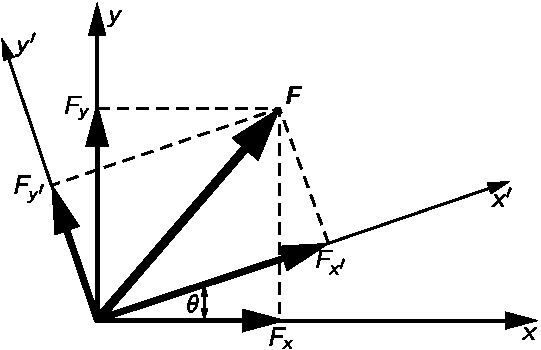
\includegraphics[width=0.8\linewidth]{fyz_fig0115.pdf}
      \caption{Složky síly ve dvou soustavách
              (\cite[s.~157]{Feynman01})}
      \label{fyz:fig0115}
    \end{figure}

    Pavel pozoruje podél svých os složky síly \(F_{x'}\), a \(F_{y'}\). \(F_{x}\) má složky ve 
    směrech \(x'\) a \(y'\) a právě tak i \(F_y\). Abychom vyjádřili \(F_{x'}\), pomocí \(F_x\) a 
    \(F_y\), sčítáme složky těchto sil podél osy \(x'\). Podobně můžeme vyjádřit \(F_{y'}\), pomocí 
    \(F_x\) a \(F_y\). Tak dostaneme
    \begin{subequations}\label{fyz:eq155}
      \begin{align}
        F_{x'} &= F_x\cos\vartheta + F_y\sin\vartheta, \label{fyz:eq155a}\\
        F_{y'} &= F_y\cos\vartheta - F_x\sin\vartheta, \label{fyz:eq155b}\\
        F_{z'} &= F_z.                                 \label{fyz:eq155c}
      \end{align}
    \end{subequations}
    Je třeba si všimnout, že vztahy (\ref{fyz:eq149}) a (\ref{fyz:eq155}) pro souřadnice \(P\) a 
    složky \(F\) \emph{mají shodný tvar}. Tato náhodná shoda má velký význam.
    
    Tak jako v přecházejícím případě, předpokládejme, že v Petrově soustavě platí Newtonovy zákony, 
    jež jsou vyjádřeny rovnicemi (\ref{fyz:eq145}). Opět se ptáme, zda Pavel může použít Newtonovy 
    zákony - zda dostane správné výsledky ve své soustavě s pootočenými osami? Jinými slovy, 
    předpokládáme-li, že rovnice (\ref{fyz:eq149}) a (\ref{fyz:eq155}) vyjadřují souvislost mezi 
    měřeními, budou, nebo nebudou správné následující vztahy?
    
    \begin{subequations}\label{fyz:eq156}
      \begin{align}
        m\dder{x'}{t} &= F_{x}, \label{fyz:eq156a}  \\
        m\dder{y'}{t} &= F_{y}, \label{fyz:eq156b}  \\
        m\dder{z'}{t} &= F_{z}. \label{fyz:eq156c}
      \end{align}
    \end{subequations}
    
    Zkoušku správnosti provedeme tak, že nezávisle vypočteme jejich levé i pravé strany a porovnáme 
    výsledky. Výpočet levých stran provádíme tak, že rovnice (\ref{fyz:eq149}) násobíme \(m\) a za 
    předpokladu, že úhel \(\vartheta\) je konstantní, dvakrát derivujeme podle času. Takovýmto 
    způsobem dostaneme
    \begin{subequations}
      \label{fyz:eq157}
      \begin{align}
        m\dder{x'}{t} &= 
          m\dder{x}{t}\cos\vartheta + m\dder{y}{t}\sin\vartheta, \label{fyz:eq157a}\\
        m\dder{y'}{t} &= 
          m\dder{y}{t}\cos\vartheta - m\dder{x}{t}\sin\vartheta, \label{fyz:eq157b}\\
        m\dder{z'}{t} &= 
          m\dder{z}{t}.                                          \label{fyz:eq157c}
      \end{align}
    \end{subequations}
    Pravé strany rovnic (\ref{fyz:eq156}) vypočteme tak, že rovnice (\ref{fyz:eq148}) dosadíme do 
    rovnic (\ref{fyz:eq155}). Tak dostaneme
    \begin{subequations}
      \label{fyz:eq158}
      \begin{align}
        F_{x'} &= m\dder{x}{t}\cos\vartheta + m\dder{y}{t}\sin\vartheta, \label{fyz:eq158a}\\
        F_{y'} &= m\dder{y}{t}\cos\vartheta - m\dder{x}{t}\sin\vartheta, \label{fyz:eq158b}\\
        F_{z'} &= m\dder{z}{t}.                                          \label{fyz:eq158c}
      \end{align}
    \end{subequations}
    
    Vida! Pravé strany rovnic (\ref{fyz:eq157}) a (\ref{fyz:eq158}) jsou shodné, a proto jsou-li
    Newtonovy zákony správné v jedné soustavě souřadnic, jsou správné i v druhé souřadnicové
    soustavě. Tento výsledek, platný pro translaci i rotaci os, má jisté důsledky. Především, nikdo
    nemůže tvrdit, že jím zvolené souřadnicové osy jsou jediné, ačkoli mohou být \emph{nejvhodnější}
    pro určitý problém. Například, je vhodné zvolit souřadnicovou soustavu tak, aby gravitační síla
    působila ve směru jedné osy, ale není to fyzikálně nezbytné. Dalším důsledkem je skutečnost, že
    každé zařízení, zcela soběstačné v tom smyslu, že obsahuje vše, co na něho silově působí, bude
    pracovat stejně při jakémkoli pootočení.
    
  \section{Vektory}\label{fyz:IchapXIsecIII}
    Nejen Newtonovy, ale pokud dnes víme i ostatní zákony fyziky mají dvě vlastnosti, jež nazýváme 
    \textbf{invariancí} (nebo symetrií) vzhledem k translaci a rotaci souřadnicových os. Tyto 
    vlastnosti jsou tak důležité, že k jejich využití při studiu fyzikálních zákonů vznikla 
    speciální matematická metoda.
    
    Předchozí analýza vyžadovala dosti pracné matematické výpočty. Aby při řešení těchto otázek 
    bylo možno omezit detailní výpočty na minimum, byl vytvořen velmi účinný matematický aparát. 
    Nazývá se \textbf{vektorová analýza} a je vlastně obsahem této kapitoly; přesně vzato však naše 
    kapitola pojednává o symetrii fyzikálních zákonů. Předcházející metody nám umožňovaly získat 
    všechny požadované výsledky, ale v praxi bychom je chtěli získat jednodušeji a rychleji, a 
    proto zavedeme vektorovou metodu.
    
    Začneme tím, že si všimneme některých rysů dvou druhů veličin, jež jsou ve fyzice důležité. (Ve 
    skutečnosti je takových druhů více, ale začneme jen se dvěma.) První druh veličin je takový, 
    jako počet brambor v pytli a tyto veličiny nazýváme obyčejnými nebo nesměřovanými čísly neboli 
    \textbf{skaláry}. Takovou veličinou je například teplota. Jiné ve fyzice důležité veličiny mají 
    směr. Je to například rychlost: Nestačí znát jen velikost rychlosti přemisťování tělesa, ale 
    musíme znát i dráhu, po níž se těleso pohybuje. I hybnost a síla mají směr, právě tak jako 
    posunutí. Když se někdo pohne z jednoho místa na druhé, můžeme zjistit, jakou dráhu urazil. 
    Chceme-li však vědět, kam šel, musíme určit směr jeho pohybu.
    
    Všechny veličiny, které mají směr (podobně jako posunutí v prostoru), nazýváme \textbf{vektory}.
    Vektor je trojice čísel. Abychom vyjádřili posunutí v prostoru, například z počátku pohybu do
    bodu \(P\), jenž má souřadnice \((x, y, z)\), skutečně potřebujeme tři čísla, ale my zavedeme
    jediný matematický symbol \(\vec{r}\), jenž se liší od dosud používaných matematických symbolů.
    \emph{Není to} jediné číslo, představuje trojici čísel: \(x, y, z\). Tento symbol představuje
    tři čísla, ale ve skutečnosti nejen \emph{tato} tři čísla, neboť při změně souřadnicové soustavy
    se ta tři čísla změní na \(x', y', z'\). Chceme však, aby naše matematika byla jednoduchá, a
    proto k označení trojice čísel \((x, y, z)\) a \((x', y', z')\) použijeme stejný znak. Použijeme
    vlastně stejný znak k vyjádření první trojice čísel v jedné souřadnicové soustavě nebo druhé
    trojice čísel v jiné souřadnicové soustavě. Tento způsob má tu výhodu, že při změně
    souřadnicového systému nemusíme měnit písmena v našich rovnicích. Zapíšeme-li rovnici pomocí
    \(x, y, z\) a pak použijeme jiný systém, musíme přejít k \(x', y', z'\), ale my budeme psát
    prostě \(\vec{r}\) a dohodneme se, že to představuje \(x, y, z\) v jednom souřadnicovém systému
    nebo \(x', y', z'\) v druhém souřadnicovém systému. Tři čísla, která popisují veličinu v dané
    souřadnicové soustavě, nazýváme \textbf{složkami} vektoru v směrech souřadnicových os
    uvažovaného systému. Používáme tedy stejný symbol pro tři písmena, která odpovídají
    \emph{stejnému předmětu v pohledu z různých os}. Skutečnost, že říkáme „stejný předmět“ se
    zakládá na fyzikální intuici o tom, že krok v prostoru nezávisí na tom, jakými složkami ho
    popisujeme. Symbol \(\vec{r}\) bude tedy představovat stejnou věc nezávisle na tom, jak otočíme
    osy.
    
    Dále předpokládejme, že existuje nějaká jiná fyzikální veličina, jež má směr, a proto je možné 
    ji určit trojicí čísel, přičemž tato tři čísla se podle určitého matematického pravidla změní 
    na tři jiná čísla při změně \((x, y, z)\) na \((x', y', z')\). Jinak řečeno, každá fyzikální 
    veličina určená trojicí čísel, jež se transformují jako složky kroku v prostoru, je vektor. 
    Rovnice typu
    \begin{equation*}
     \vec{F} = \vec{r}
    \end{equation*}
    bude správná v \emph{jakékoli} souřadnicové soustavě, je-li správná v jedné souřadnicové 
    soustavě. Tato rovnice představuje, samozřejmě, tři rovnice
    \begin{align*}
      F_x = x,     \quad F_y = y,     \quad F_z = z       \\
      \shortintertext{nebo}
      F_{x'} = x', \quad F_{y'} = y', \quad F_{z'} = z'   \\
    \end{align*}
    Skutečnost, že fyzikální závislost je možno vyjádřit pomocí vektorové rovnice, je znakem toho, 
    že závislost se nezmění otočením souřadnicové soustavy, a proto jsou vektory ve fyzice tak 
    užitečné.
    
    Nyní si všimněme některých vlastností vektorů. Jako příklady vektorů můžeme uvést rychlost, 
    hybnost, sílu a zrychlení. Často bývá vhodné znázornit vektorovou veličinu pomocí šipky, která 
    ukazuje směr jejího působení. Proč však můžeme znázornit sílu šipkou? Protože se transformuje 
    stejně jako posunutí v prostoru. Proto kreslíme sílu tak, jakoby byla posunutím a používáme 
    takové měřítko, aby jednotce síly, například jednomu newtonu, odpovídala určitá vhodná délka. 
    Jestliže jsme zavedli takovéto přiřazení, můžeme velikost všech sil vyjádřit pomocí úseček, 
    neboť rovnice typu
    \begin{equation*}
     \vec{F} = k\vec{r}
    \end{equation*}
    kde \(k\) je nějaká konstanta, je přípustná. Znázornění sil pomocí šipek je velmi výhodné, 
    neboť pak se již nemusíme starat o souřadnice. Přitom můžeme snadno vypočítat, jak se budou 
    měnit složky síly při otočení os, protože jde o geometrický problém.
    
  \section{Vektorová algebra}\label{fyz:IchapXIsecIV}
    Nyní musíme popsat zákony nebo pravidla pro různé kombinace vektorů. První takovou kombinací je 
    sčítání dvou vektorů. Nechť vektor \(\vec{a}\) má v určitém souřadnicovém systému složky \(a_x, 
    a_y, a_z\) a vektor \(\vec{b}\) složky \(b_x, b_y, b_z\). Sestavme nyní trojici nových čísel 
    \(a_x + b_x, a_y + b_y, a_z + b_z\) a zeptejme se, zda tato trojice tvoří vektor. Je možné 
    říci, že jde o trojici čísel a každá trojice čísel tvoří vektor. Pozor, ne každá tři čísla 
    tvoří vektor! Aby to byl vektor, musí jít nejen o tři čísla, ale tato čísla musí souviset se 
    souřadnicovým systémem tak, aby se při jeho otočení vzájemné „pootočila“ a „promíchala“ podle 
    zákona, o němž jsme již hovořili. Ptáme se proto, co se při takovém otočení souřadnicového 
    systému, kdy \(a_x, a_y, a_z\) přechází v \(a_{x'}, a_{y'}, a_{z'}\) a \(b_x, b_y, b_z\) v 
    \(b_{x'}, b_{y'}, b_{z'}\), stane s \(a_x + b_x, a_y + b_y, a_z + a_z\). Dostaneme pak \(a_{x'} 
    + b_{x'}, a_{y'} + b_{y'}, a_{z'} + b_{z'}\)? Odpověď na tuto otázku je kladná, protože 
    základní rovnice (\ref{fyz:eq149}) vytvářejí tzv. \emph{lineární transformaci}. Aplikujeme-li 
    takovéto transformace na \(a_x\) a \(b_x\) a vypočteme \(a_{x'} + b_{x'}\), zjistíme, že 
    transformované \(a_x + b_x\) je stejné jako \(a_{x'} + b_{x'}\). Jestliže \(\vec{a}\) a 
    \(\vec{b}\) takto „sčítáme“, dostaneme vektor \(\vec{c}\). Můžeme to zapsat takto
    \begin{equation*}
     \vec{c} = \vec{a} + \vec{b}.
    \end{equation*}
    Ze složek vektoru \(\vec{c}\), okamžitě vyplývá zajímavá vlastnost \(\vec{c} = \vec{b} + 
    \vec{a}\). Rovněž platí \(\vec{a} + (\vec{b} + \vec{c}) = (\vec{a} + \vec{b}) + \vec{c}\). 
    Vektory tedy můžeme sčítat v libovolném pořadí.
    
    \begin{figure}[ht!]  %\ref{fyz:fig0116}
      \centering
      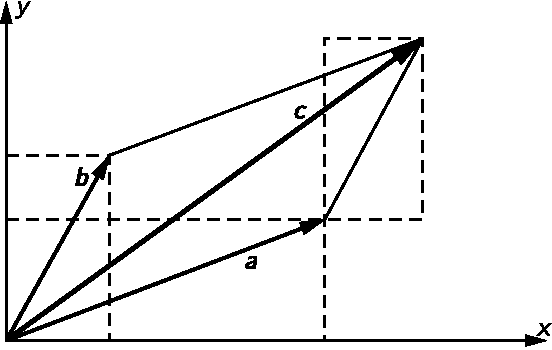
\includegraphics[width=0.8\linewidth]{fyz_fig0116.pdf}
      \caption{Sčítání vektorů
              (\cite[s.~160]{Feynman01})}
      \label{fyz:fig0116}
    \end{figure}
    Jaký je geometrický význam \(\vec{a} + \vec{b}\)? Jak bude vypadat vektor \(\vec{c}\), 
    nakreslíme-li vektory \(\vec{a}\) a \(\vec{b}\) pomocí šipek? Je to znázorněno na obr. 
    \ref{fyz:fig0116}. Vidíme, že složky vektoru \(\vec{b}\) a vektoru \(\vec{a}\) je možné 
    nejvhodněji sčítat tak, že obdélník představující složky vektoru \(\vec{b}\) přiložíme tak, jak 
    je vidět na obrázku, k obdélníku představujícímu složky vektoru \(\vec{a}\). Protože 
    \(\vec{b}\) i \(\vec{a}\) dobře „zapadnou“ do svých obdélníků, můžeme součet chápat jako 
    přiložení „chvostu“ vektoru \(\vec{b}\) k „hlavě“ vektoru \(\vec{a}\), přičemž šipka od 
    „chvostu“ vektoru \(\vec{a}\) k „hlavě“ vektoru \(\vec{b}\) je vektor \(\vec{c}\). Kdybychom 
    postupovali jinak a přiložili „chvost“ vektoru \(\vec{a}\) k „hlavě“ vektoru \(\vec{b}\), 
    dostali bychom ve shodě s geometrickými vlastnostmi obdélníků stejný výsledek pro \(\vec{c}\). 
    Všimněme si, že takovýmto způsobem sčítáme vektory bez užití souřadnicových os.
    
    Násobme vektor číslem \(\alpha\) a zkoumejme, co to znamená. Dohodněme se, že jde o nový 
    vektor, jenž má složky \(\alpha a_x, \alpha a_y, \alpha a_z\). Důkaz, že je to skutečně vektor, 
    je velmi jednoduchý.
    
    Uvažujme nyní odečítání vektorů. Odečítání můžeme definovat podobně jako sčítání, ale místo 
    sčítání složky odečítáme. Můžeme postupovat i tak, že definujeme odečítání pomocí záporného 
    vektoru \(-\vec{b}\), jenž je vlastně roven \((-1)\vec{b}\) a pak sčítání složky. Dostaneme 
    totéž. Výsledek je znázorněn na obr. \ref{fyz:fig0117}. Obrázek představuje \(\vec{d} = \vec{a} 
    - \vec{b} = \vec{a} + (-\vec{b})\). Všimněme si, že známe-li vektory \(\vec{a}\) a \(\vec{b}\), 
    můžeme snadno určit rozdíl \(\vec{a} - \vec{b}\) z ekvivalentního vztahu \(\vec{a} = \vec{b} + 
    \vec{d}\). Rozdíl se proto hledá snadněji než součet: stačí nakreslit vektor od \(\vec{b}\) k 
    \(\vec{a}\) a máme vektor \(\vec{a} - \vec{b}\)!
    

    \begin{figure}[ht!]  %\ref{fyz:fig0117}
      \centering
      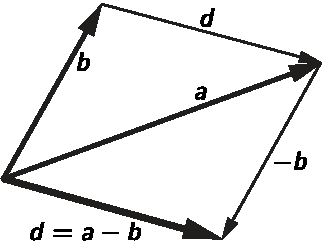
\includegraphics[width=0.7\linewidth]{fyz_fig0117.pdf}
      \caption{Odečítání vektorů
              (\cite[s.~161]{Feynman01})}
      \label{fyz:fig0117}
    \end{figure}
    Dále si všimněme rychlosti. Proč je rychlost vektor? Je-li poloha dána trojicí souřadnic 
    \((x,y, z)\), co je potom rychlost? Rychlost je určena výrazy \(dx/dt, dy/dt\) a \(dz/dt\). Je 
    to vektor, nebo není? Derivováním výrazů rovnice (\ref{fyz:eq149}) můžeme zjistit, zda se 
    \(dx'/dt\) transformuje požadovaným způsobem. Je vidět, že složky \(dx/dt\) a \(dy/dt\) se 
    transformují podle stejného zákona jako \(x\) a \(y\), i proto je časová derivace vektor. 
    Rychlost je tedy vektor. Rychlost můžeme vyjádřit zajímavým způsobem
    \begin{equation*}
      \vec{v} = \der{\vec{r}}{t}.
    \end{equation*}    
    Co je rychlost, a proč je vektor, lze také ukázat názorněji. Jak daleko se částice posune za 
    krátkou dobu \(\Delta t\)? Posune se o \(\Delta\vec{r}\), takže je-li částice v jednom okamžiku 
    „zde“ a v dalším „tam“ vektorový rozdíl poloh \(\Delta\vec{r} = \vec{r}_2 - \vec{r}_1\), jenž 
    leží ve směru pohybu (obr. \ref{fyz:fig0118}), dá po dělení časovým intervalem \(\Delta t = t_2 
    - t_1\), vektor „průměrné rychlosti“.

    \begin{figure}[ht!]  %\ref{fyz:fig0118}
      \centering
      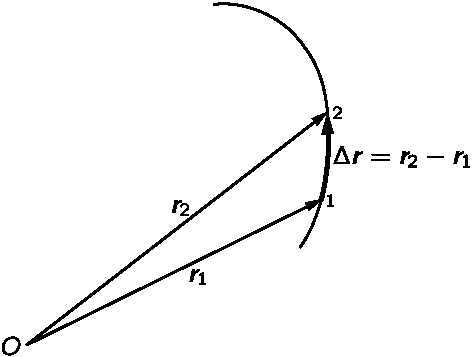
\includegraphics[width=0.8\linewidth]{fyz_fig0118.pdf}
      \caption{Posunutí částice za krátkou dobu \(\Delta t = t_2 - t_1\)
              (\cite[s.~162]{Feynman01})}
      \label{fyz:fig0118}
    \end{figure}
    Jinak řečeno, vektorem rychlostí rozumíme limitu z rozdílu polohových vektorů v okamžicích \(t 
    + \Delta t\) a \(t\) děleného \(\Delta t\), jde-li \(\Delta t\) k nule,
    \begin{equation}\label{fyz:eq154}
      \vec{v} = \lim\limits_{\Delta t\to0} = \frac{\Delta\vec{r}}{\Delta t}
              = \der{\vec{r}}{t}.
    \end{equation}
    Rychlost je tedy vektor, neboť je rozdílem dvou vektorů. Tato definice rychlostí je správná, 
    neboť složky rychlostí jsou pak \(dx/dt\), \(dy/dt\) a \(dz/dt\). Tento důkaz nám vlastně říká, 
    že derivováním libovolného vektoru podle času dostaneme nový vektor. Tak jsme poznali více 
    způsobů tvorby vektorů: (1) násobením vektoru konstantou, (2) derivováním vektoru podle času, 
    (3) sčítáním i odečítáním dvou vektorů. 

    \begin{tcnote}      
      Zapamatujme si:
      \begin{itemize}[noitemsep]
        \item Vektorem rozumíme uspořádanou trojici čísel, jejíž hodnoty závisí na volbě
              souřadnicové soustavy, tj. v různých soustavách jsou hodnoty různé.
        \item Vektor si můžeme představit jako orientovanou úsečku, kterou lze libovolně posouvat.  
        \item Vektory umíme natahovat a skládat. Obě operace provádíme po složkách. Výsledkem obou
              operací je opět vektor. 
        \item Rozdíl dvou vektorů je vektor spojující jejich koncové body. 
      \end{itemize}
    \end{tcnote}

    \subsection{Stupně abstrakce}
      V průběhu svého vývoje prošlo lidstvo třemi stupni abstrakce:
      \begin{enumerate}[leftmargin=1cm,rightmargin=.1cm, label=\emph{\alph*}),noitemsep]
        \item \textbf{oddělení čísla od předmětů.} Malé dítě počítá různé předměty: tři hrušky, dva
              domy, pět lidí. Číslo je vždy spojeno s nějakým předmětem a čtyři domy jsou něco
              jiného než čtyři limonády. V určitém věku začne ale dítě chápat číslo 4 samostatně.
              Ukáže ho na prstech a ví, že jde o čtyři výskyty jakéhokoli předmětu a netrvá již na
              tom, aby byl dotyčný předmět jmenován. V tuto chvíli si každý z nás prodělal první
              stupeň abstrakce - oddělení čísla od pojmu. Číslo nahradilo předměty.
        \item \textbf{zavedení zástupných symbolů.} Tento stupeň abstrakce jste pravděpodobně zažili
              na základní škole při počítání obsahu obdélníka. Nejprve paní učitelka kreslila různě
              veliké obdélníky na čtvercové síti a počítali jste jejich obsah podle počtu čtverečků.
              Po určité době jste se dopracovali ke vztahu S = ab. Čísla zmizela. Zůstaly zástupné
              symboly a, b pro velikost stran obdélníka a písmenko S označující jeho plochu. Čísla
              byla nahrazena proměnnými.
        \item \textbf{oddělení vlastností od matematických objektů.} Před malou chvílí jsme se
              zabývali vektory. Představili jsme si je jako tyče, které jsme se naučili natahovat a
              skládat. Ve skutečnosti jde ale o jednoduché operace s trojicemi čísel. Tyto operace
              mají zajímavé vlastnosti, které jste si mohli vyzkoušet v příkladech. Například
              složit dvě tyče a poté je natáhnout je totéž jako natáhnout každou z nich zvlášť a
              poté je složit. Ve třetím stupni abstrakce se přestaneme zabývat konkrétními
              matematickými objekty, jako byly naše pokusné tyče. Zajímat nás budou jen vlastnosti
              těchto objektů. Bude nám jedno, zda jde o tyče, jablka, matice, funkce či cokoli
              jiného. Ať je objektem cokoli, naučíme se ho natahovat a skládat s jiným podobným
              objektem tak, aby tyto operace měly stejné vlastnosti jako u tyčí, na kterých jsme si
              to vyzkoušeli.
      \end{enumerate} 

      Při třetím stupni abstrakce mizí matematické objekty a zůstávají jen vlastnosti. Hovoříme o
      zavedení tzv. \emph{lineárního vektorového prostoru}. Takovým prostorem rozumíme jakékoli
      matematické objekty (vektory, matice, funkce, řešení diferenciálních rovnic), které umíme
      natahovat a skládat tak, jako jsme to dělali s původními tyčemi. Projít si tímto stupněm
      abstrakce bude jedním z nejdůležitějších úkolů na počátku vašeho studia a bude to proces velmi
      bolestný, co se přemýšlení týče. Některým se to podaří, jiným nikoli. Těm prvním se otevře
      zcela nový svět, ve kterém budou schopni do hloubky porozumět Fourierově frekvenční analýze,
      pochopí jak hledat řešení soustav diferenciálních rovnic, jak zjednodušovat složité úlohy za
      pomoci linearizace a naučí se mnoho dalších dovedností. Ti druzí budou pasivně počítat různé
      úlohy, aniž by někdy porozuměli jejich podstatě. Pevně věřím, že u většiny z vás zvítězí touha
      po poznání nad pasivitou a probojujete se do první skupiny \cite[s.~7]{Kulhanek2020}. 
    
    \subsection{Inerciální souřadnicová soustava}
      Souřadnicová soustava, to není několik neumělých čar na tabuli. Pokud chceme opravdu měřit
      polohu těles, musíme zkonstruovat skutečnou souřadnicovou soustavu. Vezmeme si dostatečně tuhé
      tyče opatřené měřícími ryskami a svaříme z nich tři navzájem kolmé měřící osy. Už toto je
      nadlidský úkol. Tyče by se neměly prohýbat, neměly by vibrovat ani podléhat jiným deformacím.
      Zkrátka měly by to být ideálně tuhé tyče. Takové tyče ale neexistují. Pokud bychom udeřili do
      jednoho konce ideálně tuhé tyče, druhý konec by se okamžitě posunul. Informace z jednoho konce
      na druhý by se šířila nekonečnou rychlostí. A to samozřejmě není možné. Ideálně tuhé tyče tedy
      neexistují a musíme se smířit s tyčemi konečné tuhosti. Samozřejmě vybereme to nejlepší, co
      máme k dispozici, a svaříme k sobě základní trojici měřících tyčí.

      Kam ji ale umístíme? Na stůl v posluchárně. Získáme tak souřadnicovou soustavu, která bude
      sice fungovat, ale k dokonalosti bude mít daleko. Vržený předmět se v ní bude pohybovat
      nerovnoměrně a po křivce. Příčinou je naše Země, její přitažlivost a rotace. Abychom získali
      ideální soustavu, museli bychom ji umístit velmi daleko od všech těles. Tak bychom získali
      ideální soustavu, tzv. \textbf{inerciální soustavu}, ve které se tělesa budou pohybovat
      konstantní rychlostí po přímkách.

      Takový ideál ale neexistuje. Nikdy nemůžeme být dostatečně daleko od všech těles, neboť všude
      ve vesmíru nějaká tělesa jsou. Pokud se s námi v mrakodrapu utrhne výtah a poletíte volným
      pádem k zemi, nezoufejme. Na malou chvíli zažijeme skutečný inerciální systém. Pokud nám v
      údivu vypadne z ruky cokoli, daný předmět buď zůstane nehybně stát vedle nás (samozřejmě, že
      bude spolu s námi vzhledem k Zemi padat volným pádem) nebo se bude vůči nám pohybovat
      konstantní rychlostí po přímce. Volně padající klec je tedy oním ideálním inerciálním
      souřadnicovým systémem. Hovoříme o tzv. \emph{volně gravitující kleci} neboli \texttt{LIS}
      (\textbf{lokálně inerciální soustavě}). Může to být například vesmírná sonda, které došlo
      palivo. Naše souřadnicová soustava musí být ale lokální („malá“) v prostoru i v čase. Pokud by
      náš padající výtah byl veliký miliony kilometrů, vešla by se do něho Země i s Měsícem a kouzlo
      inerciální soustavy by pominulo.

      \luagraphic[1]{fyz_fig0926.png}{Experiment Harolda Waaga ukazuje jednoduchou realizaci lokální
      inerciální soustavy. (\cite[s.~8]{Kulhanek2020})}{fyz:fig0926}

      Nejlépe snad lze zavedení LIS pochopit v experimentu Harolda Waaga. Představme si tři
      propojené rovnoběžné desky s otvory na přímce. K první desce je připojeno zařízení vrhající
      kuličku, k poslední pytel, který ji zachytí. Je-li zařízení v klidu vzhledem k povrchu Země
      (stojí na Zemi, visí na laně), kulička díky tíhovému poli neproletí do pytle na pravé straně.
      Je to tím, že systém není inerciální a tělesa se nepohybují rovnoměrně přímočaře.
      Přestřihnemeli závěs a zařízení bude padat volným pádem, stává se lokálním inerciálním
      systémem (LIS), tělesa se pohybují po přímkách a kulička dopadne do záchytného pytle vpravo. 

  \twocolumn[\section{Newtonovy zákony ve vektorovém tvaru}\label{fyz:IchapXIsecV}]
    Abychom mohli zapsat Newtonovy zákony ve vektorovém tvaru, musíme provést ještě jeden malý krok 
    - definovat vektor zrychlení. Tento vektor je časovou derivací vektoru rychlosti a snadno lze 
    ukázat, že jeho složky jsou druhé derivace \(x, y\) a \(z\) podle \(t\)
    \begin{equation}\label{fyz:eq150}
      \vec{a} = \der{\vec{v}}{t} = \der{ }{t}\der{\vec{r}}{t} = \dder{\vec{r}}{t}
    \end{equation}
    \begin{align*}                   % \label{fyz:eq151}
      a_x &= \der{v_x}{t} = \dder{x}{t}, \\
      a_y &= \der{v_y}{t} = \dder{y}{t}, \\
      a_z &= \der{v_z}{t} = \dder{z}{t}.
    \end{align*}
     Pomocí této definice lze Newtonovy zákony zapsat následujícím způsobem
    \begin{equation}\label{fyz:eq152}
      \boxed{m\vec{a} = \vec{F}} \quad\text{nebo}\quad  \boxed{m\dder{\vec{r}}{t} = \vec{F}}\,.
    \end{equation}
     
     Máme dokázat, že Newtonovy zákony jsou invariantní vzhledem k otočení souřadnic. Proto musíme 
     dokázat, že \(\vec{a}\) je vektor a \(\vec{F}\) je vektor. Již jsme však dokázali, že 
     \(\vec{a}\) je vektor a o \(\vec{F}\) to budeme předpokládat. Jsou-li tedy síla i zrychlení 
     vektory, bude rovnice (\ref{fyz:eq152}) stejná ve všech souřadnicových systémech. Její zápis 
     ve tvaru, jenž explicitně neobsahuje \(x, y\) a \(z\), je výhodný proto, že chceme-li zapsat 
     Newtonovy rovnice, nebo jiné fyzikální zákony, nemusíme psát \emph{trojici} zákonů. Píšeme 
     něco, co vypadá jako jeden zákon, ale ve skutečnosti jde o tři zákony pro každý souřadnicový 
     systém, neboť každá vektorová rovnice obsahuje výrok o \emph{rovnosti jednotlivých složek}. 
     
    \begin{figure}[ht!]  %\ref{fyz:fig0119}
      \centering
      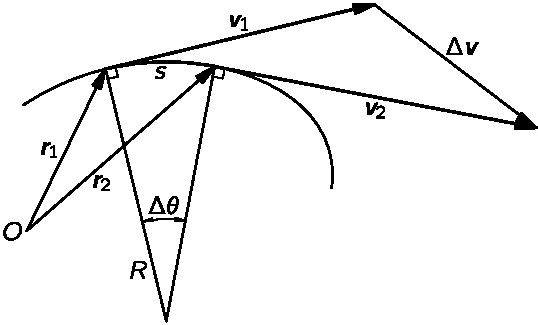
\includegraphics[width=0.9\linewidth]{fyz_fig0119.pdf}
      \caption{Křivočará trajektorie (\cite[s.~163]{Feynman01})}
      \label{fyz:fig0119}
    \end{figure}
    Skutečnost, že zrychlení je rychlost změny vektoru rychlosti, nám pomůže vypočítat zrychlení i 
    ve složitých situacích. Předpokládejme například, že částice se pohybuje po nějaké složité 
    křivce (obr. \ref{fyz:fig0119}) a v daném časovém okamžiku \(t\) má určitou rychlost 
    \(\vec{v}_1\) a v pozdějším čase jinou rychlost \(\vec{v}_2\). Jaké je zrychlení? Odpověď: 
    Zrychlení je rozdíl rychlostí dělený malým časovým intervalem. Potřebujeme tedy znát rozdíl 
    dvou rychlostí. Jak ho získáme? Kdybychom odečetli tyto dva vektory tak, že konce vektorů 
    \(\vec{v}_2\) a \(\vec{v}_1\) spojíme vektorem \(\Delta \vec{v}\), bylo by možné takto získaný 
    vektor považovat za rozdíl \(\vec{v}_2 - \vec{v}_1\)? \textbf{Ne!} Takovýmto rozdílem by byl 
    jen tehdy, kdyby počátky vektorů byly ve stejném místě. Nemá smysl takto odečítat vektory, jež 
    vycházejí z různých bodů. K jejich odečítání musíme nakreslit jiný obrázek. Na obrázku 
    \ref{fyz:fig0120} jsou \(\vec{v}_1\) a \(\vec{v}_2\) rovnoběžné a stejně velké s jimi 
    odpovídajícími vektory na obrázku \ref{fyz:fig0119}. V takovémto případě je již možné hovořit o 
    zrychlení. Zrychlení je, samozřejmě, prostě rovno \(\Delta\vec{v}/\Delta t\). Je zajímavé si 
    všimnout, že rozdíl rychlostí je možné rozložit na dvě části; je možné si představit, že 
    zrychlení má \emph{dva složkové vektory}, \(\Delta\vec{v}_1\) ve směru tečny k trajektorii a 
    \(\Delta\vec{v}_\perp\) kolmo k trajektorii (obr. \ref{fyz:fig0120}). Zrychlení, které je tečné 
    k trajektorii, vyjadřuje změnu \emph{délky} vektoru, tj. změnu \emph{velikosti rychlosti \(v\)}
    \begin{equation}\label{fyz:eq153}
      a_\parallel = \der{v}{t}.
    \end{equation}

    \begin{figure}[ht!]  %\ref{fyz:fig0120}
      \centering
      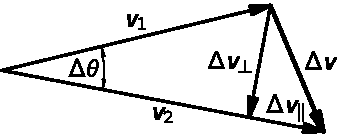
\includegraphics[width=0.8\linewidth]{fyz_fig0120.pdf}
      \caption{Diagram pro výpočet zrychlení
              (\cite[s.~163]{Feynman01})}
      \label{fyz:fig0120}
    \end{figure}
    Druhou složku zrychlení, ve směru kolmém k trajektorii je možno snadno vypočítat z obrázků
    \ref{fyz:fig0119} a \ref{fyz:fig0120}. Nechť se v krátké době \(\Delta t\) změní úhel mezi 
    \(\vec{v}_1\) a \(\vec{v}_2\) o malou hodnotu \(\Delta\vartheta\). Je-li velikost rychlosti 
    \(v\), pak je samozřejmě.    
    \begin{equation*}
      \Delta v_\perp = v\Delta\vartheta, \quad\text{a zrychlení}\quad
      a_\perp = v\frac{\Delta\vartheta}{\Delta t}.
    \end{equation*}
    Potřebujeme znát \(\Delta\vartheta/\Delta t\). Tuto veličinu je však možno najít následujícím 
    způsobem: Je-li v daném okamžiku křivka aproximována kružnicí s určitým poloměrem \(R\), pak je 
    v okamžiku \(\Delta t\) vzdálenost \(s\) rovna \(v\Delta t\), kde \(v\) je velikost rychlosti. 
    Tedy
    \begin{equation*}
      \Delta\vartheta = v\frac{\Delta t}{R}, \quad\text{neboli}\quad
      \frac{\Delta\vartheta}{\Delta t} = \frac{v}{R}.
    \end{equation*}
    Proto dostaneme vztah
    \begin{equation}\label{fyz:eq159}
      \boxed{a_\perp = \frac{v^2}{R}}\,.
    \end{equation}
    s nímž jsme se již setkali.
    
  \section{Skalární součin vektorů}\label{fyz:IchapXIsecVI}
    Skalární součin dvou vektorů \(\vec{u}\) a \(\vec{v}\) je definován jednoduchým vztahem: 
    \begin{equation*}
      \vec{u}\cdot\vec{v} \equiv u_1v_1 + u_2v_2 + u_3v_3
    \end{equation*}
    Prostě jen sečteme součiny obou prvních složek, obou druhých složek a obou třetích složek. Tři
    čárky namísto rovnítka znamenají definiční vztah. Tečka uprostřed mezi proměnnými znamená
    skalární součin. Pokud bychom tečku neuvedli, výraz by význam tenzorového součinu.

    Všimněme si ještě některých vlastností vektorů. Snadno zjistíme, že \emph{délka} posunutí v 
    prostoru je stejná v každém souřadnicovém systému. Jestliže tedy určitému posunutí \(\vec{r}\) 
    přísluší v jednom souřadnicovém systému souřadnice \(x, y, z\) a v druhém souřadnice \(x', y', 
    z'\), pak vzdálenost \(r = \abs{\vec{r}}\) musí být v obou systémech stejná. Pak
    \begin{equation*}
      r  = \sqrt{x^2+y^2+z^2}, \,\text{a}\,
      r' = \sqrt{{x'}^2+{y'}^2+{z'}^2}.
    \end{equation*}
    Chceme si ověřit, jsou-li si tyto dvě veličiny rovny. Abychom se nemuseli trápit s odmocninou, 
    uvažujme druhou mocninu vzdálenosti. Pak musíme zjistit, zda skutečně platí rovnost
    \begin{equation}\label{fyz:eq160}
      x^2+y^2+z^2 = {x'}^2+{y'}^2+{z'}^2.
    \end{equation}
    Dosadíme-li za \(x', y', z'\) vztahy (\ref{fyz:eq149}), zjistíme, že tato rovnost je splněna. 
    Takto jsme poznali jiný druh rovnic, které platí v libovolných dvou souřadnicových systémech.
    
    Setkáváme se s čím si novým. Můžeme vytvořit novou veličinu, funkci \(x, y\) a \(z\), nazvanou 
    \emph{skalární funkcí}, veličinu, která nemá směr, ale je stejná v obou systémech. Z vektoru 
    můžeme vytvořit skalár a my chceme pro tuto operaci zformulovat obecné pravidlo. Je jasné, jaké 
    bude pravidlo pro právě uvažovaný případ: je třeba sečíst druhé mocniny složek. Definujme nyní 
    novou veličinu a označme ji \(\vec{a}\cdot\vec{ a}\). Tato veličina není vektor, ale 
    \textbf{skalár}; je to číslo, které je stejné v každé souřadnicové soustavě a je definováno 
    jako součet druhých mocnin tří složek vektoru
    \begin{equation}\label{fyz:eq161}
      \vec{a}\cdot\vec{a} = {a_x}^2+{a_y}^2+{a_z}^2.
    \end{equation}
    Můžeme se zeptat: A jak je to se souřadnicovými osami? Číslo však nezávisí na volbě os, a proto 
    tento vztah platí v \emph{každé} soustavě souřadnic. Získali jsme nový \emph{druh} veličiny, 
    nový \emph{invariant} neboli skalár „umocněním“ jednoho vektoru. Definujeme-li tedy nyní pro 
    dva vektory \(\vec{a}, \vec{b}\) následující veličinu
    \begin{equation}\label{fyz:eq162}
      \vec{a}\cdot\vec{b} = a_xb_x+a_yb_y+a_zb_z.
    \end{equation}
    zjistíme, že zůstává stejná v čárkované i nečárkované soustavě souřadnic. Při důkazu tohoto 
    tvrzení můžeme využít skutečnosti, že platí pro \(\vec{a}\cdot\vec{a}\), 
    \(\vec{b}\cdot\vec{b}\) a \(\vec{c}\cdot\vec{c}\), kde \(\vec{c}=\vec{a} + \vec{b}\). Proto 
    musí být součet druhých mocnin \((a_x + b_x)^2 + (a_y + b_y)^2 + (a_z + b_z)^2\) invariantem, 
    tj.
    \begin{equation*}  %\label{fyz:eq163}
      \begin{multlined}
        (a_x + b_x)^2       + (a_y + b_x)^2       + (a_z + b_z)^2       =    \\   
        (a_{x'} + b_{x'})^2 + (a_{y'} + b_{y'})^2 + (a_{z'} + b_{z'})^2.
      \end{multlined}
    \end{equation*}
    Rozvineme-li obě dvě strany této rovnice, dostaneme takové křížové součiny jako ve vztahu 
    (\ref{fyz:eq161}) a kromě nich součty druhých mocnin složek \(\vec{a}\) a \(\vec{b}\). Protože 
    členy typu (\ref{fyz:eq161}) jsou invariantní, budou invariantní i křížové součiny typu 
    (\ref{fyz:eq162}).
    
    Veličina \(\vec{a}\cdot\vec{b}\) se nazývá skalárním součinem dvou vektorů \(\vec{a}\) a 
    \(\vec{b}\) a má mnoho zajímavých a užitečných vlastností. Například lze snadno dokázat, že
    \begin{equation}\label{fyz:eq164}
      \vec{a}\cdot(\vec{b} + \vec{c}) =  \vec{a}\cdot\vec{b} + \vec{a}\cdot\vec{c}.
    \end{equation}

    \luagraphic[1]{fyz_fig0927.pdf}{Geometrický způsob výpočtu \(\vec{a}\cdot\vec{b}\)
    (\cite[s.~9]{Kulhanek2020})}{fyz:fig0927}

    Existuje i jednoduchý geometrický způsob výpočtu \(\vec{a}\cdot\vec{b}\), při němž není třeba
    určovat složky vektorů \(\vec{a}\) a \(\vec{b}\): \(\vec{a}\cdot\vec{b}\) je součin délek
    \(\vec{a}\) a \(\vec{b}\) násobený kosinem úhlu, jež svírají vektory \(\vec{a}\) a \(\vec{b}\)
    (\ref{fyz:fig0927}). Proč? Zvolme soustavu souřadnic tak, aby její osa \(x\) ležela ve směru
    vektoru \(\vec{a}\); pak jedinou složkou \(\vec{a}\) je \(a_x=a\) a tato složka představuje i
    délku vektoru \(\vec{a}\). V takovém případě se rovnice (\ref{fyz:eq162}) redukuje na
    \(\vec{a}\cdot\vec{b} = a_x\cdot b_x\), což představuje součin délky \(\vec{a}\) a složky
    \(\vec{b}\) ve směru \(\vec{a}\), tedy \(b\cos\vartheta\).
    \begin{equation}
      \begin{aligned}\label{fyz:eq753}
        \vec{a} &= (a_x, a_y, a_z) = (a, 0, 0)  \\
        \vec{b} &= (b_x, b_y, b_z) = (b\cos\vartheta, b\sin\vartheta, 0)
      \end{aligned}
    \end{equation}
    Snadno nyní nalezneme skalární součin obou vektorů podle definice: 
    \begin{equation*}
      \vec{a}\cdot\vec{b} = (a_xb_x + a_yb_y + a_zb_z) = ab\cos\vartheta.
    \end{equation*}
    Ukázali jsme, že v takto zvolené soustavě souřadnic je \(\vec{a}\cdot\vec{b}\) součinem délek 
    \(\vec{a}\) a \(\vec{b}\) násobených \(\cos\vartheta\). \emph{Platí-li to však v jedné 
    souřadnicové soustavě, platí to ve všech souřadnicových soustavách}, neboť 
    \(\vec{a}\cdot\vec{b}\) nezávisí na volbě soustavy souřadnic.
    
    %---- Velikost a vzájemný úhel vektorů -------------------------
    % !TeX spellcheck = cs_CZ
\begin{mdframed}[style=mdexam]
  \begin{example}\label{fyz:exam026}
    Nalezněme velikost a vzájemný úhel vektorů \(\vec{a} = (1, 3, 0)\), \(\vec{b} = (2, 2, 0)\).
    \newline
    \textbf{Řešení}:  Nejprve nalezneme velikosti obou vektorů:
    \begin{align*}
      a &=\sqrt{\vec{a}\cdot\vec{a}} = \sqrt{1^2 + 3^2 + 0^0} = \sqrt{10}, \\
      b &=\sqrt{\vec{b}\cdot\vec{b}} = \sqrt{2^2 + 2^2 + 0^0} = \sqrt{8}.
    \end{align*}
    Nyní již snadno nalezneme úhel mezi oběma vektory: 
    \begin{align*}
      \cos\vartheta &= \frac{\vec{a}\vec{b}}{ab} 
                     = \frac{a_xb_x + a_yb_y + a_zb_z}{\sqrt{10}\sqrt{8}},            \\
                    &= \frac{1\cdot2 + 3\cdot2 + 0\cdot0}{\sqrt{10}\sqrt{8}} = \frac{8}{\sqrt{80}}
                       \approx\num{0.89} 
    \end{align*}
    Odpovídající úhel je přibližně \ang{27}.
  \end{example}
\end{mdframed}
    %---------------------------------------------------------------

    Je skalární součin skutečně tak užitečná veličina? Existují ve fyzice takové případy, kdy ho 
    opravdu potřebujeme? Ano, neustále ho potřebujeme. Například v kapitole \ref{fyz:IchapIV} jsme 
    nazvali kinetickou energií veličinu \(1/2 mv^2\), ale jestliže se předmět pohybuje v prostoru, 
    musíme samostatně umocnit jednotlivé složky rychlosti, takže kinetickou energii ve shodě s 
    vektorovou analýzou vyjádříme
    \begin{equation}\label{fyz:eq165}
      W_k = \frac{1}{2}m(\vec{v}\cdot\vec{v}) = \frac{1}{2}m(v_x^2 + v_y^2 + v_z^2).
    \end{equation}
    Energie nemá směr. Hybnost má směr; je to vektor představující součin hmotnosti a vektoru
    rychlosti.
    
    Jiným příkladem skalárního součinu je práce konaná silou při přemisťování předmětu z jednoho 
    místa na druhé. Zatím jsme ještě práci nedefinovali, ale je ekvivalentní změně energie při 
    zvedání závaží, když síla \(\vec{F}\) působí podél vzdálenosti \(\vec{s}\). Práce
    \begin{equation}\label{fyz:eq166}
      \vec{A} = \vec{F}\cdot\vec{s}.
    \end{equation}
    Někdy je účelné hovořit o složkách vektoru v určitém směru (například ve vertikálním směru, 
    neboť je to směr působení gravitace). V takovém případě je vhodné zavést \emph{jednotkový 
    vektor} v uvažovaném směru. Jednotkovým vektorem rozumíme takový vektor, který skalárně 
    násobený sebou samým je roven jedné. Označíme-li tento vektor \(\vec{i}\), pak platí 
    \(\vec{i}\cdot\vec{i} = 1\). Skalární součin \(\vec{a}\cdot\vec{i}\) je roven 
    \(a\cos\vartheta\), neboli složka vektoru \(\vec{a}\) ve směru \(\vec{i}\). To je výhodný 
    způsob získávání složek vektoru. Takovýmto způsobem můžeme najít všechny složky a získat dost 
    zábavný vztah. Zaveďme v daném souřadnicovém systému \(x, y, z\) tři vektory: 
    \(i\)-jednotkový vektor ve směru osy \(x\), \(j\)-jednotkový vektor ve směru osy \(y\) a 
    \(k\)-jednotkový vektor ve směru osy \(z\). Víme, že \(\vec{i}\cdot\vec{i} = 1\). Ptáme se, 
    jaké je \(\vec{i}\cdot\vec{j}\). Svírají-li dva vektory pravý úhel, jejich skalární součin je 
    roven nule. Proto
    \begin{align}
      \vec{i}\cdot\vec{i} &= 1                                      \nonumber    \\
      \vec{i}\cdot\vec{j} &= 0 \quad \vec{j}\cdot\vec{j} = 1       \label{fyz:eq167} \\
      \vec{i}\cdot\vec{k} &= 0 \quad \vec{j}\cdot\vec{k} = 0 
                               \quad \vec{k}\cdot\vec{k} = 1       \nonumber
    \end{align}
    Libovolný vektor lze tedy dá zapsat ve tvaru
    \begin{equation}\label{fyz:eq168}
      \vec{a} = a_x\vec{i} + a_y\vec{j} + a_z\vec{k}.
    \end{equation}
    Takovým způsobem můžeme přejít od složek vektoru k samotnému vektoru.
    
    Tyto úvahy o vektorech zdaleka nejsou úplné. Raději, než abychom se podrobněji zabývali touto
    problematikou, naučíme se používat některé z diskutovaných myšlenek ve fyzice. Pak, když 
    zvládneme základní materiál, bude pro nás jednodušší proniknout hlouběji do problematiky a 
    nebudeme dělat zbytečné chyby. Později poznáme, že je užitečné definovat jiný druh součinu dvou 
    vektorů, nazývaný \emph{vektorovým součinem} a označovaný symbolem \(\vec{a}\times\vec{b}\). O 
    tom však budeme hovořit až v další kapitole.
  
  \section{Vektorový součin vektorů}\label{fyz:IchapXIsecVII} 
    \emph{Vektorový součin} je operace definovaná ve vektorovém prostoru dimenze 3, do které
    vstupují dva vektory (tj. binární operace) a jejímž výsledkem je vektor na tyto dva vektory
    kolmý (viz Obr. \ref{fyz:fig0930}).

    \luagraphic[0.8]{fyz_fig0930.pdf}{Vektorový součin \(\vec{a}\times\vec{b}\)}{fyz:fig0930}

    Vektorový součin vektorů \(\vec{a}\) a \(\vec{b}\) značíme \(\vec{a}\times\vec{b}\). Výsledkem
    je vektor \(\vec{c}\), který je kolmý k \(\vec{a}\) i \(\vec{b}\). Na rozdíl od skalárního
    součinu je pořadí činitelů při vektorovém násobení důležité. Vektor \(\vec{c}\) má složky: 
    \begin{subequations}\label{fyz:eq752}
      \begin{align}
        c_1 =a_2b_3−a_3b_2,    \label{fyz:eq752a}  \\
        c_2 =a_3b_1−a_1b_3,    \label{fyz:eq752b}  \\
        c_3 =a_1b_2−a_2b_1.    \label{fyz:eq752c}
      \end{align}
    \end{subequations}
    Na první pohled vypadá tato definice možná poněkud děsivě, ale ve skutečnosti je jednoduchá.
    Stačí si zapamatovat vztah pro první složku. Po jedničce na levé straně jdou indexy dva a tři na
    pravé straně (minus obráceně). Pokud si zapamatujeme tento vztah, máme vyhráno. Vše ostatní
    dostaneme cyklickou záměnou: po jedničce jde dvojka, po dvojce trojka a po trojce zase jednička.
    Nebo po \(x\) jde \(y\), poté \(z\) a po něm zase \(x\): 

    \luagraphic[0.7]{fyz_fig0928.pdf}{Mnemotechnická pomůcka pro určení indexů složek vektorového
    součinu \(\vec{a}\times\vec{b}\) (\cite[s.~11]{Kulhanek2020})}{fyz:fig0928}

    Vektorový součin značíme křížkem, jeho výsledkem je opět trojice čísel, která má velmi podobné
    vlastnosti vektorům. Někdy tomuto útvaru říkáme \textbf{pseudovektor}. Budeme se jím ještě
    mnohokrát abývat, například až budeme probírat rotace v prostoru (kapitola \ref{fyz:IchapXX}).

    Zobecněním vektorového součinu pro prostory dimenze \(n\) je tzv. \textbf{ortogonální doplněk}
    \(n-1\) vektorů, operace, do níž vstupuje \(n − 1\) vektorů a jejímž výsledkem je jeden vektor
    na všechny tyto vektory kolmý.

    %---- Vektorový součin -----------------------------------------
    % !TeX spellcheck = cs_CZ
\begin{mdframed}[style=mdexam]
  \begin{example}\label{fyz:exam027}
    Nalezněme vektorový součin vektorůů \(\vec{a} = (1, 2, 3)\), \(\vec{b} = (4, 5, 6)\).
    \newline
    \textbf{Řešení}: Vyjdeme přímo z definice:
    \begin{align*}
      \vec{a}\times\vec{b} 
        &\equiv  (a_2b_3−a_3b_2, a_3b_1−a_1b_3, a_1b_2−a_2b_1)                      \\
        &= (2\cdot6-3\cdot5, 3\cdot4-1\cdot6, 1\cdot5-2\cdot4)                      \\
        &= (3, 6, 3). 
    \end{align*}
  \end{example}
\end{mdframed}
    %---------------------------------------------------------------
    
    Jsou-li vektory \(\vec{a}\) a \(\vec{b}\) rovnoběžné, ať již souhlasně či nesouhlasně, je
    \(\vec{a}\times\vec{b} = 0\). Velikost vektoru \(\vec{a}\times\vec{b}\) (píšeme
    \(\abs{\vec{a}\times\vec{b}}\)) nabývá největší možné hodnoty, jsou-li vektory \(\vec{a}\) a
    \(\vec{b}\) \emph{kolmé}.

    \begin{figure}[ht!]  %\ref{fyz:fig0929}
      \centering
      \subcaptionbox{\label{fyz:fig0929a}}{\luafigure[0.45]{fyz_fig0929a.pdf}}
      \subcaptionbox{\label{fyz:fig0929b}}{\luafigure[0.45]{fyz_fig0929b.pdf}}
      \caption{Pravidlo pravé ruky pro vektorový součin. (a) Natočme pravou ruku
              tak, aby vektor \(\vec{a}\) byl ve směru ukazováčku a \(\vec{b}\) ve směru
              prostředníku. Pak palec ukazuje směr \(\vec{c} = \vec{a}\times\vec{b}\). (b) Vidíme,
              že \((\vec{a}\times\vec{b}) = -(\vec{a}\times\vec{b})\).(\cite[s.~50]{Halliday2001})}
      \label{fyz:fig0929}
    \end{figure}

    Obr. \ref{fyz:fig0929b} ukazuje použití pravidla pravé ruky při určení směru vektoru \(\vec{c}' =
    \vec{a}\times\vec{b}\). Prsty nyní směřují od \(\vec{b}\) k \(\vec{a}\) a palec ukazuje opačným
    směrem, než na obr. \ref{fyz:fig0929a}. Vektor \(\vec{c}'\) je tedy opačný k vektoru \(\vec{c}\),
    \(\vec{c}' = −\vec{c}\). Platí tedy 
    \begin{equation}\label{fyz:eq755}
      \vec{b}\times\vec{a} = −(\vec{a}\times\vec{b}).
    \end{equation}
    Pro vektorový součin \emph{neplatí komutativní zákon}.  

    Nalezněme nyní význam vektorového součinu. K tomu použijeme stejnou souřadnicovou soustavu, jako
    tomu bylo u skalárního součinu, tj. vektory budou mít složky (\ref{fyz:eq753}). Pro vektorový
    součin potom podle definice (\ref{fyz:eq752}) vyjde \((0\cdot0−0\cdot b\sin\vartheta,
    0\cdot b\sin\vartheta−a\cdot0, ab\sin\vartheta−0\cdot b\sin\vartheta)\) pouze \(z\)-ová
    souřadnice nenulová:
    \begin{equation}\label{fyz:eq754}
      \vec{a}\times\vec{b} = (0,0,ab\sin\vartheta) 
    \end{equation}
    Vektorový součin má složku jen v ose \(z\), tedy míří kolmo na oba původní vektory (obr.
    \ref{fyz:fig0930}). Jeho velikost je rovna \(ab\sinα\), tj. ploše rovnoběžníku „nataženého“ na
    oba vektory. 

    \begin{tcnote}      
      Určení směru vektorového součinu \(\vec{a}\times\vec{b}\) můžeme také použít vývrtky na špunty
      (obr. \ref{fyz:fig0931}). Pokud otočíme vektorem \(\vect{a}\) směrem k \(\vect{b}\) po
      nejkratší dráze, šroub se zavrtává proti směru hodinových ručiček, tj. v kladném směru osy
      \(z\). Myšlený pohyb provádíme vždy s vektorem, který je uveden jako první.

      {\centering
        \captionsetup{type=figure} 
        \luafigure[1]{fyz_fig0931.pdf}
        \captionof{figure}{Pravidlo pravé ruky a vývrtky}
        \label{fyz:fig0931}
      \par}
    \end{tcnote}

  \section{Příklady a cvičení}\label{fyz:IchapXIsecVIII}
    %---------------------------------------------------------------
      % !TeX spellcheck = cs_CZ
\begin{example}\label{fyz:fey_exam012}
  Dvě síly stejné velikosti \SI{250}{\newton} svírají úhel \ang{60}. Určete velikost výslednice.
      
  {\centering
   \captionsetup{type=figure}
   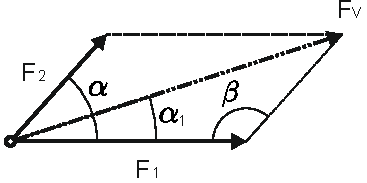
\includegraphics[width=0.5\linewidth]{fyz_fig380.pdf}
   \captionof{figure}{Grafické určení výslednice dvou sil se společným působištěm, svírajících 
     \(\alpha\). Také platí \(\beta = \ang{180}-\alpha\) a pak \(\cos\beta = - \cos\alpha_1\) 
   \label{fyz:fig380}}
  \par}
  
  Velikost síly \(F_v\) můžeme určit graficky pomocí vektorového rovnoběžníku. Velikosti sil 
  \(F_1\) a \(F_2\) vyneseme ve zvoleném měřítku (např. \SI{50}{\newton} = \SI{1}{\cm}), vykreslíme 
  rovnoběžník dle obrázku a délku uhlopříčku převedeme zpět ve stejném měřítku na velikost síly 
  \(F_v\). Početně určíme velikost výslednice pomocí kosinové věty: 
  \begin{align*}
     F_v^2 &= F_1^2 + F_2^2 - 2F_1F_2\cdot\cos\beta \\
     F_v^2 &= F_1^2 + F_2^2 - 2F_1F_2\cdot\cos(\ang{180}- \alpha) \\
     F_v   &= \sqrt{2F_1^2 - 2F_1^2\cdot\cos(\ang{180}- \alpha)}  \\
         &= \sqrt{2}F_1\sqrt{1-\cos(\ang{180}- \alpha)}         \\
         &= \sqrt{2}\cdot250\sqrt{1-\cos(\ang{180} - \ang{60})} 
            \cong \SI{433}{\newton}
  \end{align*}

\end{example}
    %---------------------------------------------------------------
    %---------------------------------------------------------------
      % !TeX spellcheck = cs_CZ
% Marsak, Havrankova - Sbirka resenych prikladu z fyziky - Termika a molekulova fyzika.pdf
\begin{example}\label{fyz:fey_exam011}
  Lampa o hmotnosti \SI{5}{\kg} visí uprostřed dlouhého původně vodorovného drátu a způsobí jeho 
  prohnutí o \ang{1} od vodorovného směru (viz obr. \ref{fyz:fig379}). Určete velikost síly \(F_n\)
  napínající drát. 
      
  {\centering
   \captionsetup{type=figure}
   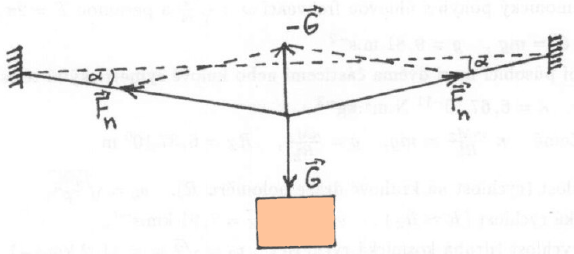
\includegraphics[width=0.7\linewidth]{fyz_fig379.png}
   \captionof{figure}{K příkladu \ref{fyz:fey_exam011} \cite[s.~6]{Havrankova1995}
   \label{fyz:fig379}}
  \par}
  
  Tíhová síla, kterou lampa prohýbá drát musí být vyrovnána vertikální silou vzniklou jako 
  výslednice napěťových sil působících v drátu. Tedy
  \begin{equation*}
     G = 2F_n\sin\alpha = mg, \quad m = \SI{5}{\kg}, \quad
     \sin\alpha = \sin\ang{1} \approx \alpha = \num{0.017}
  \end{equation*}
  \begin{equation*}
    F_n = \frac{mg}{2\sin\alpha} = \frac{\num{5}\cdot\num{9.81}}{2\cdot\num{0.017}}
        = \SI{1443}{\newton}
  \end{equation*}
  \begingroup\makeatletter\def\f@size{7}\check@mathfonts
  \def\maketag@@@#1{\hbox{\m@th\large\normalfont#1}}%
    \begin{align*}
      \shortintertext{\footnotesize Použitý vzorec můžeme snadno odvodit z kosinové věty:}
      G &= \sqrt{F_1^2 + F_2^2 - 2F_1F_2\cdot\cos2\alpha} \\
      \shortintertext{\footnotesize s přihlédnutím, že obě síly jsou si rovny a s využitím  
        goniometrického vzorce pro dvojnásobný úhel \(\cos2\alpha = \cos^2\alpha - \sin^2\alpha\) 
        můžeme provést následující úpravy} 
      G &= \sqrt{2F_n^2\cdot(1-\cos2\alpha)}=\sqrt{2}F_n\sqrt{1-\cos^2\alpha+\sin^2\alpha}  \\
        &=\sqrt{2}F_n\sqrt{2\sin^2\alpha} = 2F_n\sin\alpha
    \end{align*}
  \endgroup
  Drát bude napínán stejnou silou, jako kdyby na něj působilo tahem těleso tíhy \SI{1443}{\newton}, 
  tedy o hmotnosti \SI{147}{\kg}
\end{example}
    %---------------------------------------------------------------
%---------------------------------------------------------------------------------------------------